\subsection{Les organes}
\label{sec:organes}
\subsubsection{La carte réseau}
\label{sec:CarteReseau}
Un ordinateur (ou n'importe quel appareil informatique) communique via sa carte réseau. C'est elle qui fait l'interface entre l'ordinateur et le réseau en lui-même.

Lorsque votre ordinateur communique sur le réseau, c'est en réalité sa carte réseau qui le fait. De même, les paquets (messages) sont adressés à cette carte réseau.

Chaque carte réseau possède un identifiant \textbf{unique} appelé \textbf{adresse MAC}. C'est sa carte d'identité, ce qui l'identifie au sein d'un réseau. Nous en reparlerons quand nous parlerons du protocole de communication Ethernet.

\begin{figure}[h]
\centering
  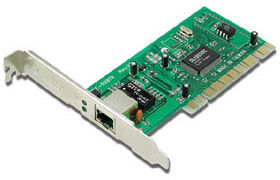
\includegraphics[width=.4\textwidth]{images/materiel/carteReseau}
  \caption{Carte réseau}
  \label{fig:carteReseau}
\end{figure}

\subsubsection{Concentrateur (hub)}
\label{sec:concentrateur}
Un concentrateur est un dispositif qui permet de relier différents organes (ordinateurs) entre-eux. Chaque organe est relié sur un port (prise RJ45) différent. On peut le voir comme une simple "multi-prise" qui se contente d'envoyer tout ce qu'elle reçoit sur un port sur les autres ports.

Par exemple, si quatre ordinateurs sont connectés sur les ports 1, 2, 3 et 4 et que l'ordinateur branché sur le port 4 envoie un paquet à celui connecté sur le port 2, le hub le transmettra sur les ports 1, 2 et 3 sans se soucier du destinataire du message.

\subsubsection{Commutateur (switch)}
\label{sec:commutateur}
Un commutateur sert également à relier différents organes entre-eux au sein d'un réseau. Cependant, contrairement au concentrateur, le commutateur ne recopie pas tous les messages qu'il reçoit sur tous les ports. En effet, il n'enverra le paquet uniquement au port sur lequel est connecté son destinataire.

En reprenant l'exemple précédent, lorsque l'ordinateur connecté au port 4 désire envoyer un paquet à celui connecté au port 2, le commutateur transmettra ce message sur le port 2 et non sur les autres ports.

Pour identifier les éléments connectés sur ses ports, le commutateur utilise l'adresse MAC (l'identifiant unique attribué aux cartes réseaux).

\subsubsection{Routeur}
\label{sec:routeur}
Un routeur, quant à lui, permet non seulement de connecter des organes entre-eux, mais il fait également le lien entre deux réseaux différents. L'exemple le plus parlant est sûrement la box internet que chacun à chez soi. Elle permet de relier les différents ordinateur du domicile entre-eux et permet également à ces ordinateur d'accéder à un réseau bien plus étendu : internet.


\subsection{On récapitule}

Le tableau~\ref{tab:materiel} (issu du site OpenClassRooms) regroupe les différents materiels abordés et leur fonctions principales.

\begin{table}[h!t]
\centering
  \begin{tabular}{l|p{.6\textwidth}}
  \textbf{Matériel} & \textbf{Fontion} \\\hline
  Carte réseau & La carte réseau est le matériel de base indispensable, qui traite tout au sujet de la communication dans le monde du réseau.\\\hline

Concentrateur (hub) & Le concentrateur permet de relier plusieurs ordinateurs entre eux, mais on lui reproche le manque de confidentialité. On peut le voir comme une simple «multi-prise» Ethernet. \\\hline

Commutateur (switch) & Le commutateur fonctionne comme le concentrateur, sauf qu'il transmet des données aux destinataires en se basant sur leurs adresses MAC (adresses physiques). Chaque machine reçoit seulement ce qui lui est adressé.\\\hline

Routeur & Le routeur permet d'assurer la communication entre différents réseaux pouvant être fondamentalement différents (réseau local et Internet).\\\hline

Répéteur& Le répéteur reçoit des données par une interface de réception et les renvoie plus fort par l'interface d'émission. On parle aussi de relais en téléphonie et radiophonie.\\
\end{tabular}

  \caption{Récapitulatif des matériels abordés}
  \label{tab:materiel}
\end{table}
